\documentclass{beamer}
%
\mode<presentation>
{
  \usetheme{default}      % or try Darmstadt, Madrid, Warsaw, ...
  \usecolortheme{default} % or try albatross, beaver, crane, ...
  \usefonttheme{default}  % or try serif, structurebold, ...
  \setbeamertemplate{navigation symbols}{}
  \setbeamertemplate{caption}[numbered]
} 

\usepackage[english, russian]{babel}
\usepackage[utf8x]{inputenc}
\usepackage{color}

\title[Course presentation]{Challenges and perspectives in machine learning}
\author{Alexis Zubiolo\newline\texttt{alexis.zubiolo@gmail.com}}
\institute{Data Science Team Lead @ Adcash}
\date{February 16, 2017}

\begin{document}

\begin{frame}
  \titlepage
\end{frame}

\begin{frame}{Purpose of this talk}
Illustrate recent \textbf{trends} and \textbf{challenges} in machine learning on \textbf{practical examples}.
\end{frame}

\begin{frame}
\center
\Huge
\textbf{Supervised learning paradigm}
\end{frame}

\begin{frame}{Supervised learning paradigm}
~\\
\textbf{Goal}: Build algorithms that can 
\begin{itemize}
	\item \textbf{learn} from data
	\item \textbf{make predictions} on data
\end{itemize}
\vfill
\pause
\begin{figure}
\centering
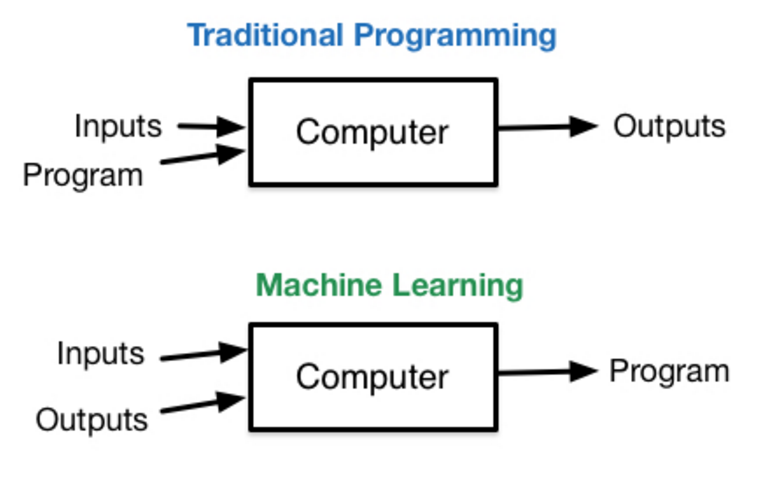
\includegraphics[width=\textwidth]{images/ml_vs_traditional.png}
\end{figure}
\end{frame}

\begin{frame}
\center
\Huge
\textbf{Example 1: Machine translation}
\end{frame}

\begin{frame}{Machine translation}
Machine learning is a way to perform automated translation:
\begin{itemize}
	\item Input = reference text
	\item Output = translated text
\end{itemize}
\pause
\vfill
There are differences between languages at different levels:
\begin{itemize}
	\item Genders, e.g. neutral, masculine, feminine
	\item Conjugation
	\item Cases
	\item \dots
\end{itemize}
\end{frame}

\begin{frame}{Machine translation: A tricky example}
Take a close look at these two sentences:
\pause
\vfill
The trophy could not fit in the bag because \textbf{it} is too small. \\
\vfill
and
\vfill
The trophy could not fit in the bag because \textbf{it} is too big. \\
\pause
\vfill
What does the word "\textbf{it}" refer to in both cases?
\end{frame}

\begin{frame}{Machine translation: A tricky example}
Take a close look at these two sentences:
\vfill
The trophy could not fit in {\color{blue}\textbf{the bag}} because {\color{blue}\textbf{it}} is too small. \\
\vfill
and
\vfill
{\color{red}\textbf{The trophy}} could not fit in the bag because {\color{red}\textbf{it}} is too big. \\
\vfill
What does the word "\textbf{it}" refer to in both cases?
\end{frame}

\begin{frame}{Machine translation: A tricky example}
Based on the context, we can guess what "\textbf{it}" refers to.
\vfill
\pause
This is key because, if we wanted to translate this sentence into Bulgarian, we would be faced to the following challenge:
\begin{itemize}
	\item {\color{red}Trophy = трофей} is {\color{red}masculine}
	\item {\color{blue}Bag = чанта} is {\color{blue}feminine}
\end{itemize}
\vfill
\pause
\textbf{Consequence}: "it" would refer to a masculine or a feminine noun, depending on the context.
\end{frame}

\begin{frame}{Machine translation: A tricky example}
Let's translate this sentence \textbf{from English to Bulgarian}... Here is my attempt:
\pause
\vfill
The trophy could not fit in the {\color{blue}\textbf{bag}} because {\color{blue}\textbf{it}} is too small. \\ \pause
= Трофеят не може да се побере в {\color{blue}\textbf{чантата}}, защото ({\color{blue}\textbf{тя}}) е твърде {\color{blue}\textbf{малка}}.
\pause
\vfill
The {\color{red}\textbf{trophy}} could not fit in the bag because {\color{red}\textbf{it}} is too big. \\ \pause
= {\color{red}\textbf{Трофеят}} не може да се побере в чантата, защото ({\color{red}\textbf{той}}) е твърде {\color{red}\textbf{голям}}.
\pause
\vfill
This is often referred to as \textbf{long short-term memory} (LSTM).
\end{frame}

\begin{frame}{Another example}
Classic challenge in machine translation: \textbf{homonyms}.
\vfill
\pause
\textbf{Example}:
\pause
\vfill
\begin{figure}
\centering
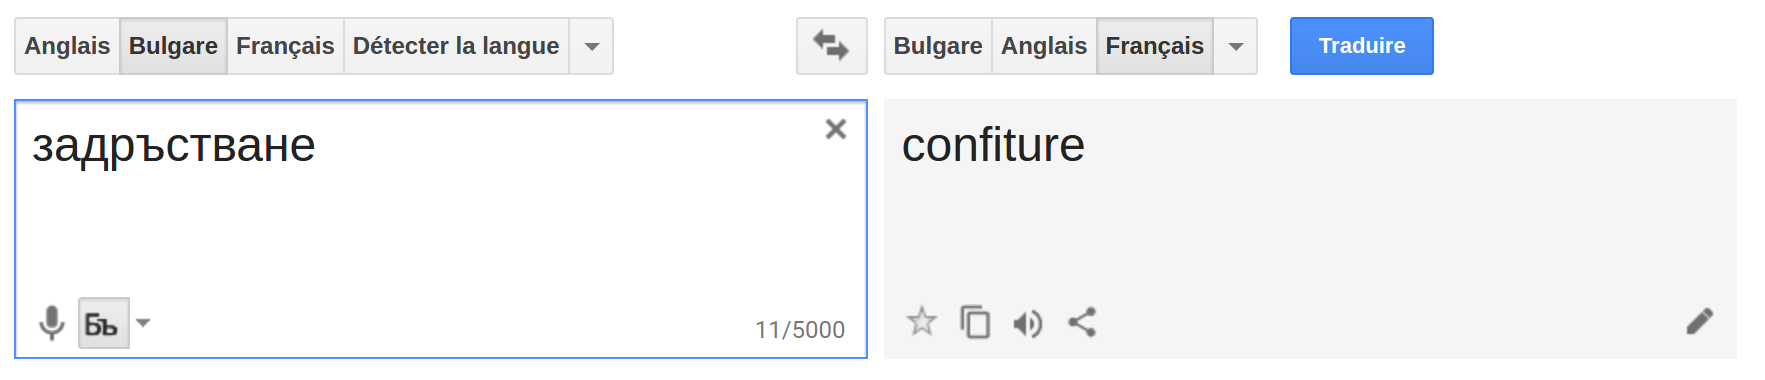
\includegraphics[width=\textwidth]{images/jam_google_translate.png}
\end{figure}
\pause
\vfill
\begin{figure}
\centering
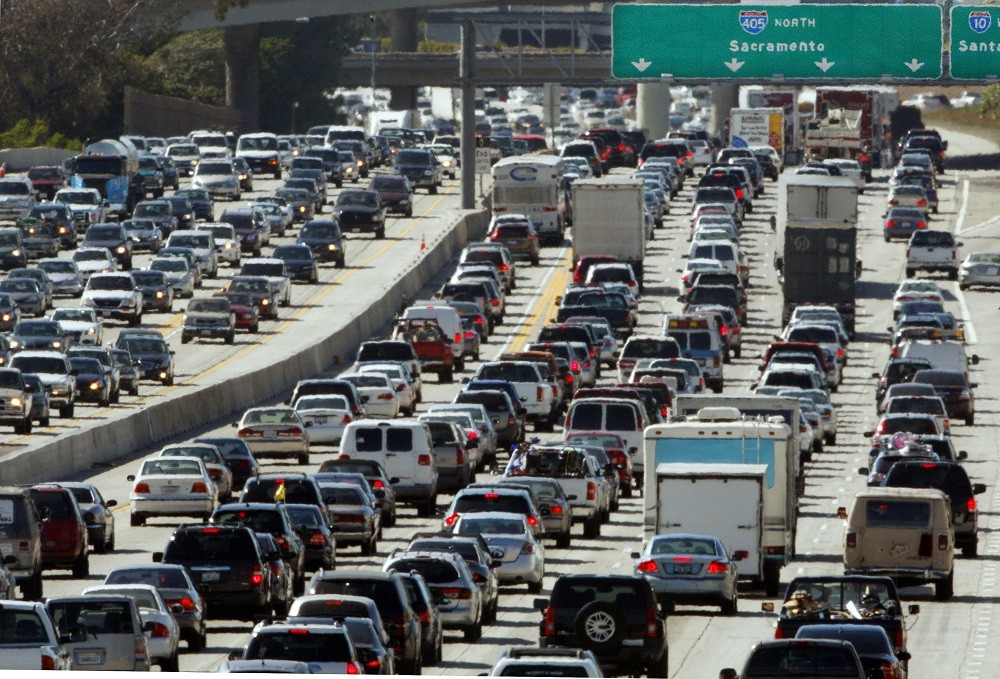
\includegraphics[width=.45\textwidth]{images/traffic_jam.jpeg}~
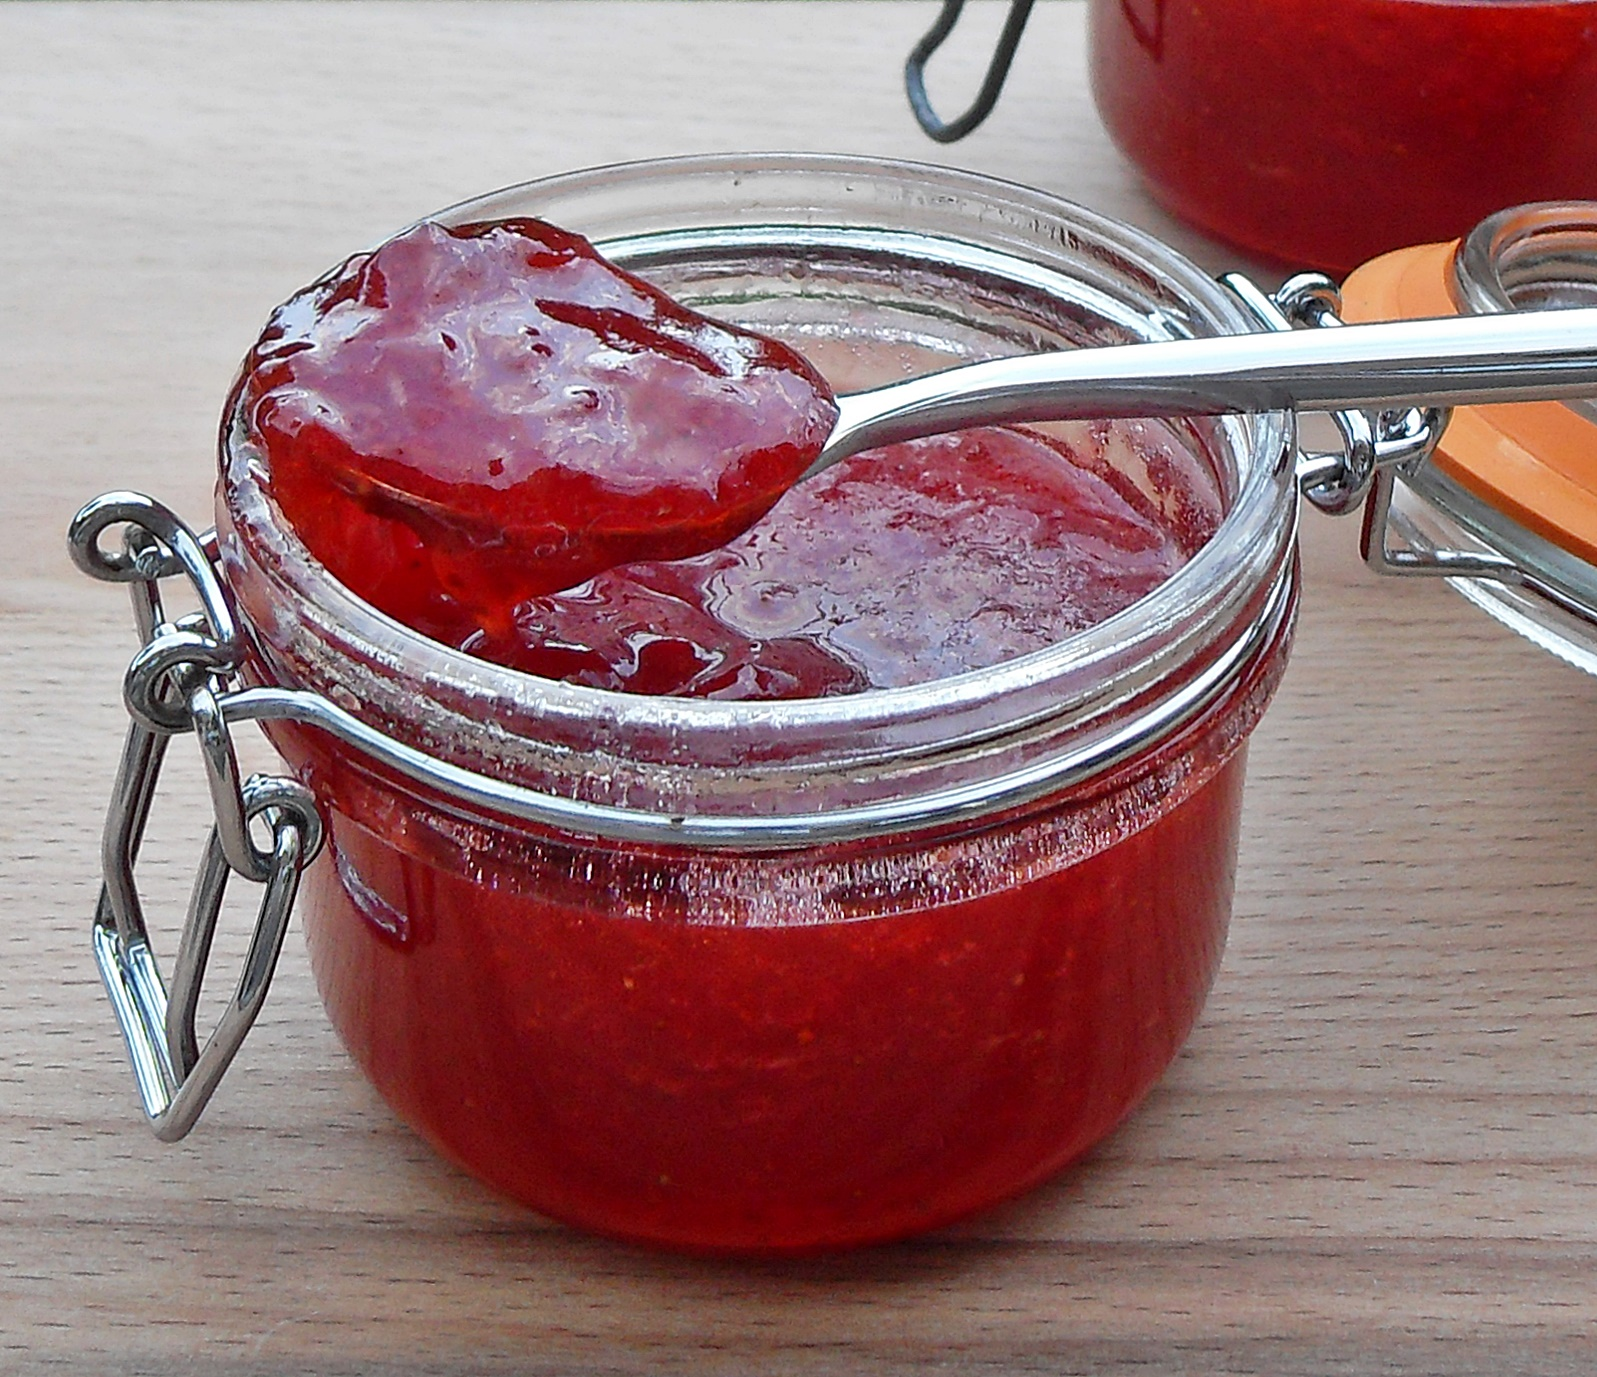
\includegraphics[width=.4\textwidth]{images/jam.jpg}
\end{figure}
\pause
\vfill
How could it be? \pause This is \textbf{jam} in English.
\end{frame}

\begin{frame}
\center
\Huge
\textbf{Example 2: Acquiring data}
\end{frame}

\begin{frame}{Acquiring data}
Let us switch to another example: \pause Reading house numbers in Google street.
\pause
\vfill
\begin{figure}
\centering
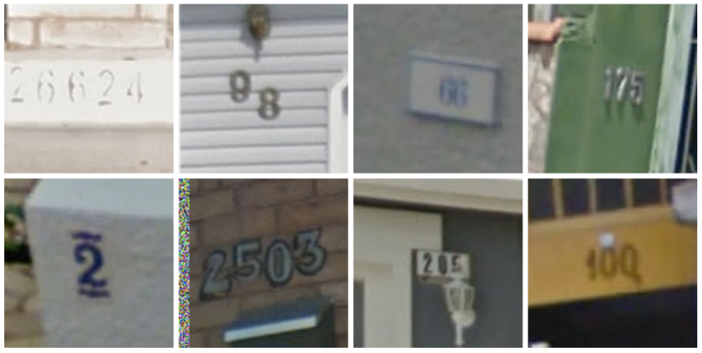
\includegraphics[width=\textwidth]{images/street_numbers.png}
\end{figure}
\end{frame}

\begin{frame}{Acquiring data}
Why would we do that? \pause In order to locate houses accurately.
\vfill
\pause
\begin{figure}
\centering
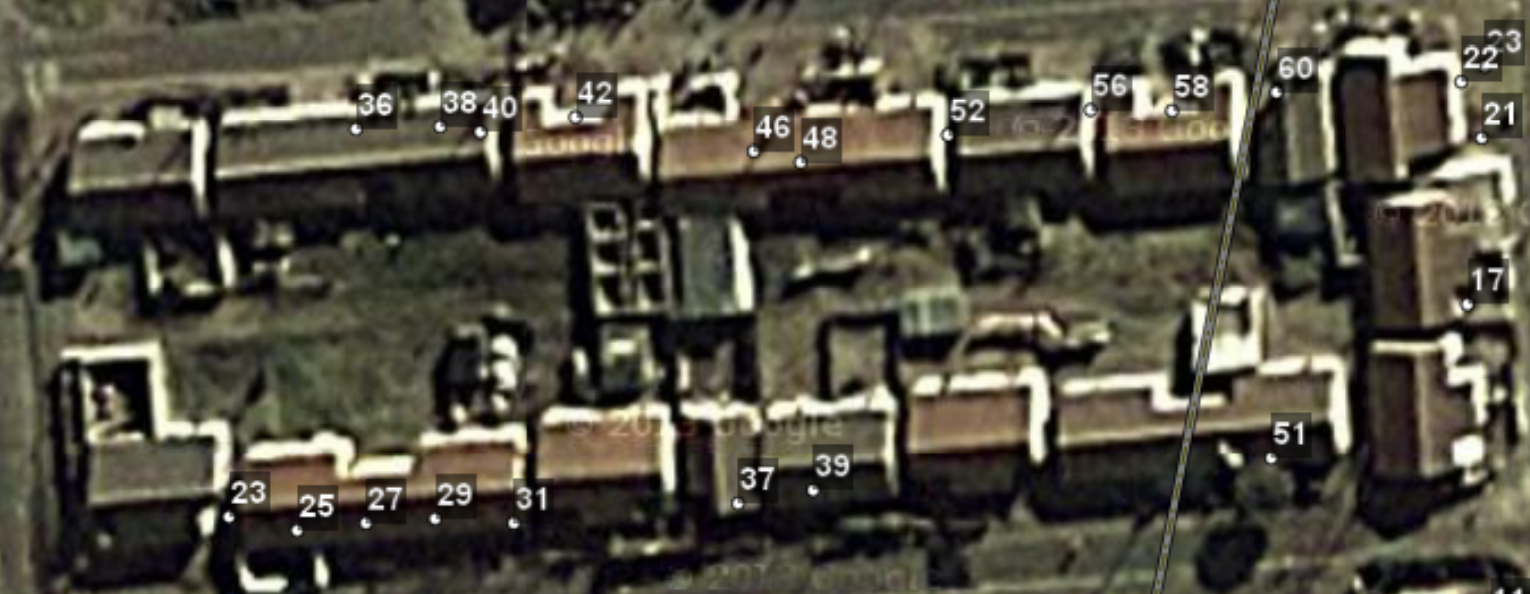
\includegraphics[width=\textwidth]{images/house_numbers.png}
\end{figure}
\end{frame}

\begin{frame}{Acquiring data}
There exist really good machine learning algorithms to read numbers automatically but \ldots \pause They need \textbf{training data}, that is:
\begin{itemize}
	\item inputs (images with numbers on it): They \textbf{already have} \pause
	\item outputs (value): They \textbf{don't have}
\end{itemize}
\vfill
\pause
What did they do to obtain this labelled data? \pause Propose a free \textbf{CAPTCHA} system \ldots
\vfill
\pause
\begin{figure}
\centering
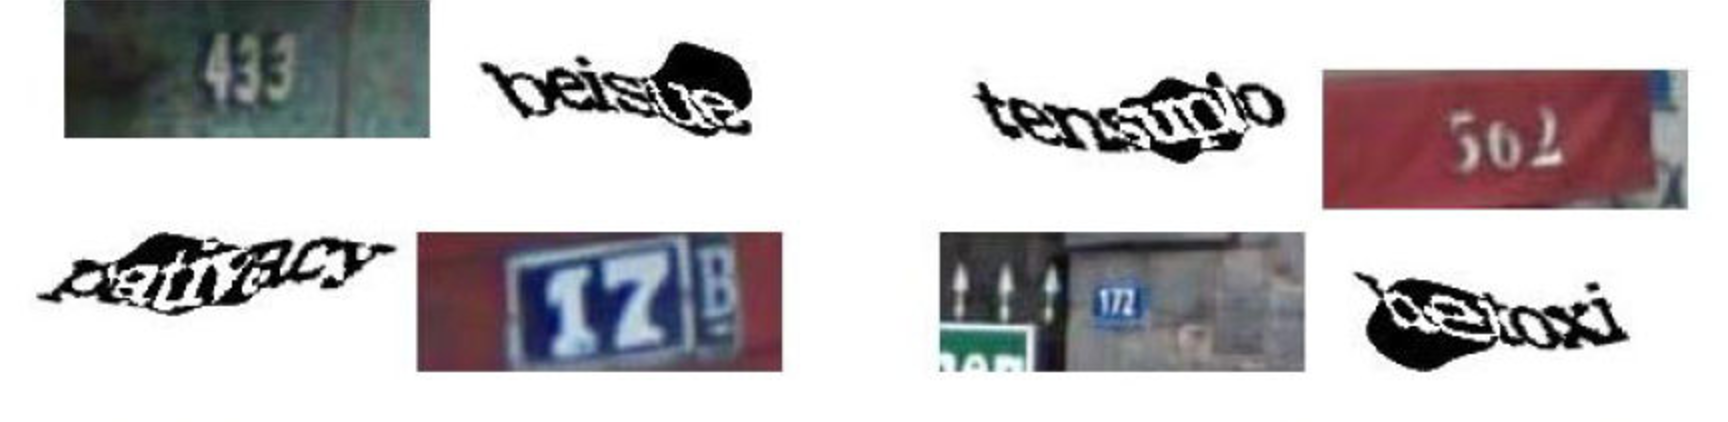
\includegraphics[width=\textwidth]{images/captchas.png}
\end{figure}
\vfill
\pause
\ldots so that real human can provide labels (outputs) to their images (inputs)!
\end{frame}

\begin{frame}{Conclusion}
Machine learning is not only about designing super sophisticated algorithms (even if it helps!).
\vfill
\pause
Gathering \textbf{a significant amount of (clean) data} is \textbf{crucial}!
\vfill
\pause
Understanding \textbf{corner cases} is \textbf{key}!
\end{frame}

\begin{frame}
\vfill
\centering
\begin{huge}
\huge{Thank you! Questions?}
\vfill
\texttt{alexis.zubiolo@gmail.com}
\end{huge}
\vfill
\end{frame}

\end{document}
